\section{K5 -- Ocena złożoności algorytmów}

\textbf{Złożoność algorytmu} jest miarą ilości zasobów potrzebnych do rozwiązania danego problemu o określonym rozmiarze. Dla przykładu w algorytmie rozkładu liczb na czynniki pierwsze zauważyć można, że im większa liczba, tym dłużej będziemy ją rozbijać i wykonamy więcej obliczeń. Faktem zatem jest, że im większy rozmiar danych wejściowych, tym więcej zasobów potrzebujemy do rozwiązania problemu. Złożoność algorytmu można więc określić mianem \textbf{funkcji rozmiaru danych wejściowych}.

Wyróżnić możemy kilka \textbf{klas złożoności}, czyli grup zagadnień o podobnej złożoności obliczeniowej. Są to:
\begin{enumerate}
	\item \textbf{NP} (\textit{nondeterministic polynomial}) - problemy decyzyjne rozwiązywalne niedeterministycznym algorytmem wielomianowym.
	\item \textbf{P} (\textit{deterministic polynomial}) - problemy decyzyjne, które można rozwiązać deterministycznym algorytmem o złożoności wielomianowej.
	\item \textbf{NP-zupełny} - problemy decyzyjne, których znalezienie rozwiązania nie jest możliwe w czasie wielomianowym.
	\item \textbf{NP-trudny} (silnie NP-zupełny) - samo sprawdzenie rozwiązania problemu jest co najmniej tak trudne jak każdego innego problemu NP.
\end{enumerate}

\begin{figure}[!h]
\centering
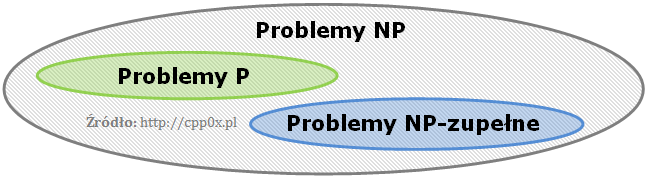
\includegraphics[width=0.6\textwidth]{k5_zbior_problemow_np.png}
\caption{Klasy złożoności}
\end{figure}

Aby określić złożoność stosowane są metody \textbf{oceny złożoności}. W celu ujednolicenia wyników i uniezależnienia się od środowiska, ocena złożoności rozpatrywana jest modelem abstrakcyjnym nie uwzględniającym platformy czy mocy obliczeniowej maszyny. Wyróżniamy następne modele złożoności:
\begin{enumerate}
	\item \textbf{Czasowe} - czas wykonywania algorytmu wynikająca z liczby operacji elementarnych wykonywanych podczas przebiegu programu.
	\item \textbf{Pamięciowe} - pamięcio-żerność oraz zasobo-żerność - ilość pamięci operacyjnej, bądź przestrzeni dyskowej potrzebnej do rozwiązania problemu. Zależy od liczby oraz złożoności użytych struktur.
\end{enumerate}

Przy wyborze algorytmu zazwyczaj decydująca jest złożoność czasowa - o wiele bardziej miarodajny model.

Wyróżniamy także podział złożoności algorytmów ze względu na instancję problemu:
\begin{enumerate}
	\item \textbf{Optymistyczna} - najlepszy możliwy przypadek (minimalna ilość wykonywanych operacji).
	\item \textbf{Pesymistyczna} - najgorszy scenariusz (wykonywane są wszystkie operacje).
	\item \textbf{Średnia} - wartość oczekiwana wykonywania algorytmu.
\end{enumerate}

Do oceny złożoności algorytmu potrzebny jest \textbf{rząd wielkości} oraz zmienność zależnie od instancji problemu. Nie potrzebne są dokładne wartości, dlatego też stosuje się \textbf{asymptotyczne tempo wzrostu}, które to informuje nas o zmianie (wzroście bądź spadku) złożoności algorytmu w zależności od ilości danych wejściowych. Opisuje jak szybko funkcja rośnie, maleje, bądź pozostaje stała.

Asymptotyczne tempo wzrostu określane jest za pomocą \textit{notacji asymptotycznych}. Istnieje kilka notacji \textit{Bachmann-Landaua}:
\begin{itemize}
	\item $\mathcal{O}$ (omikron, duże O)  - Funkcja asymptotycznie \textbf{niewiększa}. Jest to ograniczenie górne, czyli taka funkcja, dla której wszystkie wartości funkcji badanej, będą od niej niewiększe (mniejsze bądź równe).
	\item $\Omega$ (omega) - Funkcja asymptotycznie \textbf{niemniejsza}. Jest to granica dolna, czyli funkcja, dla której wszystkie wartości funkcji badanej, będą od niej niemniejsze (większe bądź równe).
	\item $\Theta$ (theta) - Funkcja asymptotycznie \textbf{podobna}. Jest to oszacowanie dokładne, czyli funkcje ograniczające badaną funkcję od góry i od dołu.
	\item $o$ - (małe O) - Funkcja asymptotycznie mniejsza. Rzadko stosowana.
	\item $\omega$ - (mała omega) - Funkcja asymptotycznie większa. Rzadko stosowana.
\end{itemize}

Złożoności kategoryzuje się do rzędów złożoności. Określają one jak szybko złożoność algorytmu rośnie wzraz ze wzrostem instancji problemu.

\begin{figure}[!h]
\centering
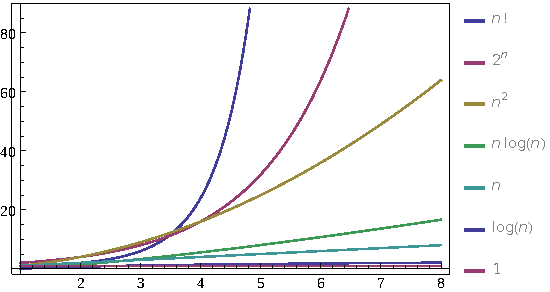
\includegraphics[width=0.8\textwidth]{k5_wykres_wszystkie.pdf}
\caption{Porównanie rzędów złożoności}
\end{figure}

Wyróżnić można (\textit{n - liczba danych wejściowych}):
\begin{itemize}
	\item $\mathcal{O}(1)$ - \textbf{złożoność stała} -  liczba operacji jest niezależna od rozmiaru problemu. Przykład: Ustalenie, czy liczba binarna jest dodatnia bądź ujemna, obliczenie $(-1)^n$, odwołanie się do n-tego elementu stałej w rozmiarze tablicy.
	\item $\mathcal{O}(\log n)$ - \textbf{logarytmiczna} - liczba operacji rośnie proporcjonalnie do logarytmu z rozmiaru problemu. Przykład: Wyszukiwanie binarne w posortowanej tablicy, dodanie/usunięcie elementu z drzewa binarnego.
	\item $\mathcal{O}(n)$ - \textbf{liniowa} - liczba operacji jest wprost proporcjonalna do rozmiaru problemu. Przykład: Znalezienie min/max elementu w nieposortowanej tablicy, dodanie dwóch n-bitowych liczb całkowitych w sumatorze z przeniesieniem szeregowym.
	\item $\mathcal{O}(n\log n)$ - \textbf{quasi-liniowa} - liczba operacji proporcjonalna do iloczynu rozmiaru problemu i jego logarytmu. Sortowania przez porównania (MergeSort (przez scalenie), HeapSort (kopcowe), QuickSort (szybkie)), FFT (Szybka Transformata Fouriera).
	\item $\mathcal{O}(n^2)$ - \textbf{kwadratowa} - liczba operacji rośnie proporcjonalnie do kwadratu rozmiaru problemu. Przykład: Prosty algorytm mnożenia dwóch n-bitowych liczb, sortowania: BubbleSort (bąbelkowe), SelectionSort (przez wybieranie), InsertionSort (przez wstawianie), znalezienie najkrótszej ścieżki w grafie.
	\item $\mathcal{O}(n^k)$ - \textbf{wielomianowa} - liczba operacji rośnie proporcjonalnie do wielomianu rozmiaru problemu. Przykład: Programowanie liniowe, maksymalne skojarzenie dla grafu dwudzielnego.
	\item $\mathcal{O}(2^n)$ - \textbf{wykładnicza} - liczba operacji rośnie proporcjonalnie do wartości wykładniczej rozmiaru problemu. Przykład: Programowanie dynamiczne dla problemu komiwojażera.
	\item $\mathcal{O}(n!)$ - \textbf{rzędu silnia} - liczba operacji rośnie proporcjonalnie do silni rozmiaru problemu. Przykład: Algorytm brute-force dla problemu komiwojażera.
\end{itemize}
